\documentclass[12pt, a4paper]{article}
\usepackage[utf8]{inputenc}
\usepackage[T2A]{fontenc}
\usepackage{indentfirst, setspace}
\usepackage{tabularx, multirow}
\usepackage[normalem]{ulem}
\usepackage[style=russian]{csquotes}
\usepackage[english,russian]{babel}
\usepackage{hyperref}
\usepackage{ragged2e}
\usepackage{caption}
\usepackage{wrapfig}
\usepackage{amsmath}
\usepackage{tikz}
\makeatletter
\def\@biblabel#1{#1. }
\makeatother
\captionsetup{labelsep=endash}
\usepackage{listings}
\linespread{1.3}
\lstset{
  language=C++,
  basicstyle=\ttfamily\small,
  keywordstyle=\color{blue},
  breaklines=true,
  commentstyle=\color{green},
  stringstyle=\color{red},
  extendedchars=\true,
  showstringspaces=false,
  keepspaces=true,
}

\usepackage[left=2cm,right=2cm,
    top=2cm,bottom=2cm,bindingoffset=0cm]{geometry}\begin{document}
\begin{titlepage}
     \fontsize{12}{12}\selectfont

  {\centering

   \begin{bf}

    \begin{wrapfigure}{l}{10mm}
        
\includegraphics[width=17mm]{photo_2023-12-23.jpeg}
    \end{wrapfigure}


    \noindent Министерство науки и высшего образования Российской Федерации

    \noindent Федеральное государственное бюджетное образовательное учреждение высшего образования

    \noindent \enquote{Московский государственный технический университет

     \noindent имени Н.Э. Баумана

     \noindent (национальный исследовательский университет)}

    \noindent (МГТУ им. Н.Э. Баумана)

   \end{bf}
  }

  \vspace{0.4cm}

  {\setstretch{0.1}
   \noindent\rule{\textwidth}{1mm}
   \noindent\rule{\textwidth}{0.5mm}

  }

  \fontsize{14}{21}\selectfont

  \noindent\begin{tabularx}{\textwidth}{l >{\centering\arraybackslash}X}
   ФАКУЛЬТЕТ & \flqq Фундаментальные Науки\frqq \\ \cline{2-2}

   КАФЕДРА & ФН-12 \flqq Математическое моделирование\frqq \\ \cline{2-2}
  \end{tabularx}

  \vspace{1cm}


  \begin{center}
   \begin{bf}

    \fontsize{24}{36}\selectfont
    ОТЧЕТ

    \fontsize{20}{30}\selectfont
    ПО ЛАБОРАТОРНОЙ РАБОТЕ НА ТЕМУ:

    Обход графовых структур

   \end{bf}
  \end{center}

  \fontsize{14}{21}\selectfont
  \vspace{5cm}


  \noindent\begin{tabularx}{\textwidth}{ X >{\centering}p{4cm} p{1cm} c }
   Студент: & & & Мациевский И. М. \\ \cline{2-2} \cline{4-4}
   & \fontsize{10}{15}\selectfont дата, подпись & & \fontsize{10}{15}\selectfont Ф.И.О. \\
   Преподаватель: & & & Волкова Л. Л.\\ \cline{2-2} \cline{4-4}
   & \fontsize{10}{15}\selectfont дата, подпись & & \fontsize{10}{15}\selectfont Ф.И.О.
   \end{tabularx}

  \vspace{\fill}

  \begin{center}
   \it{Москва}, 2023
  \end{center}

  \thispagestyle{empty}
\end{titlepage}\newpage
\tableofcontents
\newpage
\section*{Введение}
\addcontentsline{toc}{section}{Введение}
\justifying
\textbf{Цель лабораторной работы}: реализовать алгоритмы обхода графовых структур.

Для достижения поставленной цели требуется решить следующие \textbf{задачи}.
\begin{enumerate}
\item Описать граф и бинарное дерево.
\item Реализовать графовую структуру.
\item Реализовать возможность пользователю самостоятельно заполнять графовую структуру.
\item Реализовать обход графовой структуры в ширину и в глубину.
\item Выполнить тестирование реализации разработанного алгоритма.
\end{enumerate}

Согласно варианту, требуется разработать бинарное дерево.

\newpage
\section{Аналитическая часть}
\textbf{Граф ---} это абстрактная структура данных, представляющая собой набор 
вершин (узлов) и рёбер, соединяющих их. 

\textbf{Граф с петлями ---} граф, в котором рёбра могут соединять вершину с 
самой собой, а также быть кратными, то есть соединять одни и те же 
вершины несколько раз.

\textbf{Бинарное дерево} --- это иерархическая структура данных в виде дерева, в 
которой каждый узел может иметь не более двух дочерних узлов: левый и правый. У 
дерева есть две главные характеристики:
\begin{enumerate}
    \item Корень --- верхний узел дерева, от которого начинаются все другие 
    узлы. У бинарного дерева может быть только один корень.
    \item Листья --- узлы без дочерних узлов называются листьями. Листья 
    находятся на самом нижнем уровне дерева.
\textbf{Обход в глубину ---} алгоритм обхода графа или дерева, начиная с 
выбранной вершины и продвигаясь максимально вглубь, прежде чем возвращаться к 
предыдущей вершине. В процессе обхода отмечаются посещенные вершины.
\textbf{Обход в ширину ---} алгоритм обхода графа или дерева, начиная с 
выбранной вершины и постепенно расширяясь на смежные вершины одного уровня перед 
переходом к следующему уровню. В процессе обхода отмечаются посещенные вершины.
\end{enumerate}
\newpage
\section{Конструкторская часть}
\textbf{Бинарное дерево}
\begin{enumerate}
	\item \textbf{Создание корня дерева:} Пользователь вызывает функцию 
	$addElementToTree()$. Вводится значение для корня дерева, которое затем 
	становится корнем нового узла.
	\item \textbf{Метод $addElementToTree()$} добавляет элемент в дерево: 
	Создается узел с введенным значением и устанавливается как корень дерева.
	Вызов вспомогательной функции addElement(root) для добавления левого и 
	правого потомка корня.
	\item \textbf{Метод $addElement$} Запрос у пользователя для добавления 
	левого узла к текущему узлу. Если ответ "да", то вводится значение для 
	левого узла, создается новый узел и устанавливается в качестве левого 
	потомка текущего узла. Затем рекурсивно вызывается $addElement$ для левого 
	потомка. Аналогичные шаги для правого узла.
	\item \textbf{Вывод результатов:} Вызываются методы $printBreadthTree()$ и 
	$printDepthFirstTree()$ для вывода элементов дерева в ширину и в глубину 
	соответственно.
\end{enumerate}
\textbf{Обход в ширину $BreadthTree$:}
\begin{enumerate}
	\item Проверяет, является ли переданный узел нулевым. Если да, то 
	возвращается.
	\item Иначе, создается очередь $nodesQueue$, и корень дерева помещается в 
	очередь.
	\item В цикле, пока очередь не пуста, извлекается передний узел очереди.
	\item Выводится значение текущего узла.
	\item Если у текущего узла есть левый потомок, он добавляется в очередь.
	\item Если у текущего узла есть правый потомок, он также добавляется в 
	очередь.
\end{enumerate} 
\newpage
Блок-схема представлена на рис.~\ref{img:grap1}.
	\begin{figure}[h]
  		\center{\includegraphics[scale=1]{block1}}
  		\caption{Блок-схема обхода в ширину}
  		\label{img:grap1}
	\end{figure}

\textbf{Обход в глубину $DepthTree$:}
\begin{enumerate}
	\item Проверяет, является ли переданный узел нулевым. Если да, то 
	возвращается.
	\item Иначе, создается стек (nodesStack), и корень дерева помещается в стек.
	\item В цикле, пока стек не пуст, извлекается верхний узел стека.
	\item Выводится значение текущего узла.
	\item Если у текущего узла есть правый потомок, он добавляется в стек.
	\item Если у текущего узла есть левый потомок, он добавляется в стек.
\end{enumerate}
\newpage
Блок-схема представлена на рис.~\ref{img:grap2}.
	\begin{figure}[h]
  		\center{\includegraphics[scale=1]{block2}}
  		\caption{Блок-схема обхода в глубину}
  		\label{img:grap2}
	\end{figure}
\newpage
\section{Технологическая часть}
Для реализации выбран язык C++.
На листинге 1 представлена реализация программы
(Реализация~\ref{lst:label1})
\begin{lstlisting}[caption={Исходный код}, label={lst:label1}]
#include <iostream>
#include <string>
#include <queue>
#include <stack>

using namespace std;

template <typename T>
class BinaryTreeNode {
public:
    T data;
    BinaryTreeNode<T>* left;
    BinaryTreeNode<T>* right;

    BinaryTreeNode(T value) : data(value), left(nullptr), right(nullptr) {}
};

template <typename T>
class BinaryTree {
private:
    BinaryTreeNode<T>* root;

    void addElement(BinaryTreeNode<T>* node) {
        string choice;

        cout << "Добавить значение в левый узел для узла " << node->data << "? (да/нет): ";
        cin >> choice;

        if (choice == "да") {
            T value;
            cout << "Введите значение для левого узла: ";
            cin >> value;
            node->left = new BinaryTreeNode<T>(value);
            addElement(node->left);
        }
        else if (choice == "нет") {
            node->left = nullptr;
        }

        cout << "Добавить значение в правый узел для узла " << node->data << "? (да/нет): ";
        cin >> choice;

        if (choice == "да") {
            T value;
            cout << "Введите значение для правого узла: ";
            cin >> value;
            node->right = new BinaryTreeNode<T>(value);
            addElement(node->right);
        }
        else if (choice == "нет") {
            node->right = nullptr;
        }
    }

    void BreadthTree(BinaryTreeNode<T>* node) {
        if (node == nullptr) {
            return;
        }

        queue<BinaryTreeNode<T>*> nodesQueue;
        nodesQueue.push(node);

        while (!nodesQueue.empty()) {
            BinaryTreeNode<T>* current = nodesQueue.front();
            nodesQueue.pop();
            cout << current->data << " ";

            if (current->left != nullptr) {
                nodesQueue.push(current->left);
            }
            if (current->right != nullptr) {
                nodesQueue.push(current->right);
            }
        }
    }

    void DepthTree(BinaryTreeNode<T>* node) {
        if (node == nullptr) {
            return;
        }

        stack<BinaryTreeNode<T>*> nodesStack;
        nodesStack.push(node);

        while (!nodesStack.empty()) {
            BinaryTreeNode<T>* current = nodesStack.top();
            nodesStack.pop();
            std::cout << current->data << " ";

            if (current->right != nullptr) {
                nodesStack.push(current->right);
            }
            if (current->left != nullptr) {
                nodesStack.push(current->left);
            }
        }
    }

public:
    BinaryTree() : root(nullptr) {}

    void addElementToTree() {
        T value;
        cout << "Введите значение для корня дерева: ";
        cin >> value;
        root = new BinaryTreeNode<T>(value);
        addElement(root);
    }

    void printBreadthTree() {
        cout << "Обход дерева в ширину: ";
        BreadthTree(root);
        cout << endl;
    }

    void printDepthFirstTree() {
        cout << "Обход дерева в глубину: ";
        DepthTree(root);
        cout << endl;
    }
};

int main() {
    setlocale(0, "");
    BinaryTree<int> binaryTree;
    binaryTree.addElementToTree();
    cout << endl;
    binaryTree.printBreadthTree();
    cout << endl;
    binaryTree.printDepthFirstTree();
    return 0;
}
\end{lstlisting}
\newpage
\begin{center}
	\textbf{Примеры работы}
\end{center}
На рисунках примеры работы программы.
\begin{enumerate}
	\item Входные файлы: граф, состоящий из переменных типа $char$.
	Результат приведён на рис.~\ref{img:grap3}.
	\begin{figure}[h]
  		\center{
\includegraphics[scale=0.7]{ex1.png}}
  		\caption{Пример работы 1}
  		\label{img:grap3}
	\end{figure}
	\newpage
	\item Входные файлы: граф, состоящий из переменных типа $int$.
	Результат приведён на рис.~\ref{img:grap4}.
	\begin{figure}[h]
  		\center{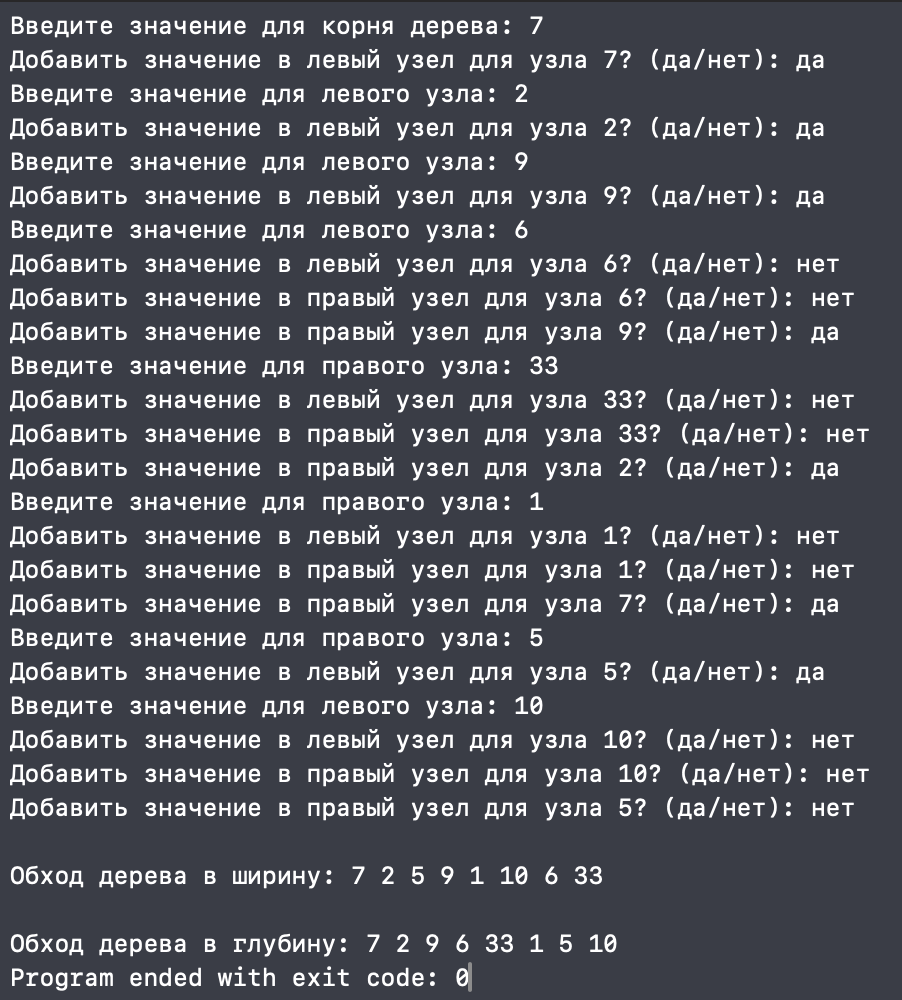
\includegraphics[scale=0.7]{ex2.png}}
  		\caption{Пример работы 2}
  		\label{img:grap4}
	\end{figure}
\end{enumerate}
\newpage
\section*{Заключение}
\addcontentsline{toc}{section}{Заключение}
Цель лабораторной работы достигнута: реализован алгоритмы обхода бинарного дерева.

В результате выполнения лабораторной работы были выполнены все задачи.
\begin{enumerate}
\item Описано бинарное дерево.
\item Программно реализовано бинарное дерево.
\item Реализована возможность пользователю самостоятельно заполнять бинарное дерево.
\item Реализован обход бинарного дерева в ширину и в глубину.
\item Выполнено тестирование реализации разработанного алгоритма.
\end{enumerate}
\newpage
\begin{center}
\begin{thebibliography}{}
\addcontentsline{toc}{section}{Список используемых источников}
\bibitem{book}Буркатовская Ю.Б., Теория графов. Часть 1: учебное пособие Томский 
политехнический университет. – Томск: Изд-во Томского политехнического 
университета, 2014. – 200 с.
\end{thebibliography}
\end{center}
\end{document}